\documentclass[conference]{IEEEtran}

\usepackage{datetime}
\usepackage{cite}
\usepackage[pdftex]{graphicx}
\usepackage{epstopdf}
\usepackage[utf8]{inputenc}
\usepackage{amsfonts}
\usepackage{amssymb}
\usepackage{graphicx}
\usepackage{tikz}
\usepackage{float}
\usepackage{color}
\usepackage{subfig}
\usepackage[hyphens]{url}

\hyphenation{}

\newcommand{\xcloud}{x-cloud}
\newcommand{\Xcloud}{X-cloud}

\begin{document}

\title{Performance and mobility in the \xcloud}

% author names and affiliations
% use a multiple column layout for up to three different
% affiliations
\author{
\IEEEauthorblockN{Jakub Krzywda}
\IEEEauthorblockA{Dept. of Computing Science\\Umeå University\\
SE-901 87 Umeå, Sweden\\
Email: jakub@cs.umu.se}
\and
\IEEEauthorblockN{William Tärneberg}
\IEEEauthorblockA{Dept. of Electrical and Information Technology\\Lund University\\
Ole Römers väg 3, 223 63 Lund, Sweden \\
Email: william.tarneberg@eit.lth.se}}

\maketitle

\begin{abstract}
%\boldmath
In an \xcloud topology the resources are dispersed throughout the network. Given that services strictly migrate with the user from, depending on the placement of the service hosts, user mobility will affect the performance perceived performance of the service. The model takes into account the effort of migrating a service and the service performance degradation it introduces.

This paper determines the fundamental service performance issues in system of mobile users with disperead data centres, in relation to the placement of the \xcloud host nodes and explores the user and provider utility of subscribing to an \xcloud node at a certain network depth.
\end{abstract}

\IEEEpeerreviewmaketitle

\section{Introduction}
Mobile services and \ue functions are at an increasing rate beeing virtualized and augmented to the cloud. Applications are soon more ofthen than not seamliessly executed, partially or fully in the cloud. Alongside applications, fundemental \ue resources, such as storage and CPU, are being virtualized to the cloud. In this paradigm, the border between what is beeing executed locally and remotely is blurred as developers are given more powerful tools to tap into remote ubiquitous generic virtual resources. This resource paradigm, has overwhelmingly augmented the capabilities of mobile applications, and enabled collaborateive computing. In the years to come, just short of all devices will contribute data to the cloud and\/or utilize its resources.

As we begin to rely more on remote resources we also grow more dependant on the communication delay introduced by the the intermediate WAN network and by the geographical separation of the \ue and the \dc. Latency sensitive applications such as process controlls, latency sensitive storage, real time video game rendering, and augmented reality video analysis will quickly faulter if subject to a significant and varying communication delay.

The virtual resources are accessed through increasingly congested mobile access networks. More devices are crowding the mobile networks and applications generating and receiving more data, this congestion translates into delay. Additionally, the geographic distance to the data centre introduces a propagation delay, bounded by the speed of light.

The \xcloud paradigm, put forward by \cite{chandra2013decentralized,ericsson_akami}, attemps to remedy the aformentioned congestion and latency by locating cloud resources at the edged of and adjacent to the mobile access networks. In the ad-hoc scenario, resources are shared amongst \ues as each \ue surrenders its availbale resources generically to its peers. However, from a network perspective, at one extreme \dc resources can propsedly be located in at the edge of the network, adjacent or integrated into an \rbs, catering for the \ues reciding within its cell. Alternatively, or complimenarty, \dcs can be integrated with resources in the proposed forthcoming virtualized radio access networks. The scale and the degree of dispersion can be optimized for each application, given the applications resource tiers and its users mobility behaviour.

The geograpghic proximity between the \ue and the \dc is proportional to application service delay, to that effect, services hosted in the \xcloud are migrated with the \ue, through the network, to minimize this incurred latency. In practice, services, or rather the VMs that host the services will be migrated to the node that is available, provides the lowest delay, and incurrs least global network congestion. However, by doing so might minimize the experiance delay for the \ue, but will incurr a migration overhead in \dc and in the network a VM is migrated. Conceivably, various schemes and cost functions can be deployed to minimize both the delay experianced by the user and the added resource strain to th \dc and the network.

The topology paradigms of tomorrows all-ap mobile networks all-IP (Internet Protocol) \cite{6144211,5357099} are yet to be determined, but one can assume that they will be influenced by the notion of virtualized resources \cite{baroncelli2010network, chowdhury2009network}. Large portions of \rbss can proposedly be virtualized and centrallized to a common local-geographic \dc, shared by several \rbss, leaving the \rbss, in principal, with just the radio interface \cite{melzercloud}. The expanse of the centralization is geographically bounded by propagation delay and signal attenudation, and is resource hampered by the aggregate traffic that passes through the dedicated \dc. There is extensive research directed at exploring relevant economic and IT models \cite{EricssonWhitePaper,6156350, 5357099}.

The concept of geo-disributed cloud resources has been worked on for a few years, but with a clear focus on storage and sharded data. The authors of \cite{agarwal2010volley} pressent a method to geographically migrate shared data resouces globaly, not only to minimize the distance between the \ue and the \dc, and thus service latency, but also to globaly load-balance the hosting \dcs. Their results reveal a significant reduction in service latency, inter-\dc communication, and contributed WAN congestion. Their proposed controll process runs over longer periods of time and operate on a global scale with georgraphically static users. Although sharing some fundamental dynamisc, ableit at different scales, in contrast, in the \xcloud paradigm, \ue movement is much more rapid and proportional to the size of a session. Additinally, \xcloud virtualized resources are assumed to be universal and do not just cover data, and vary in size and capabilities.

The field of \xcloud bears much in common with geo-disributed cloud resources but is dominated by the notions of augmenting \ues through virtualizing their resources \cite{6563280} and reducing service response times through geo-cascaded data caching \cite{1437087,ericsson_akami}. As a result, much of the research is concerned with coping with specific dynamics, and do thus not address the generic case of generic locally geo-distributed resouces serving a local subscriber populous. There is large amount of work left to explore the fundamental dynamics of the \xcloud in order to be able to begin to consider specific applications and use-cases.

\Ue mobility is a key differentiator between traditional distant immobile clouds and the \xcloud, and is a fundamental dynamic property of an \xcloud. It is therefore essential to understand how \ue mobility affects the perceived service performance and what load it imposes on the network in the generic case.

This paper contributes with models designed to examine the fundamental and generic resource problems in an \xcloud of mobile \ues. The models include a generic mobile network inhabited by \ues subscribing to a number of services, served by a number of locally geo-distributed \dcs.

This paper provides an investigation into the fundamental effects of user \ue in the \xcloud in relation to the number of subscribers, the abstract placement of the servers, and the numer of services. An optimal or reasonable technical bounds for the \xcloud topology is not yet to be determined. This paper disregards the deeper techincal and topological constrains of existing mobile systems in order to provide fundamental resulst that can be employed to shape the forthcoming mobile nework generations.

%------------------------------------------------------------------

\section{Desiard model}

\begin{figure}[tb]
	\centering
	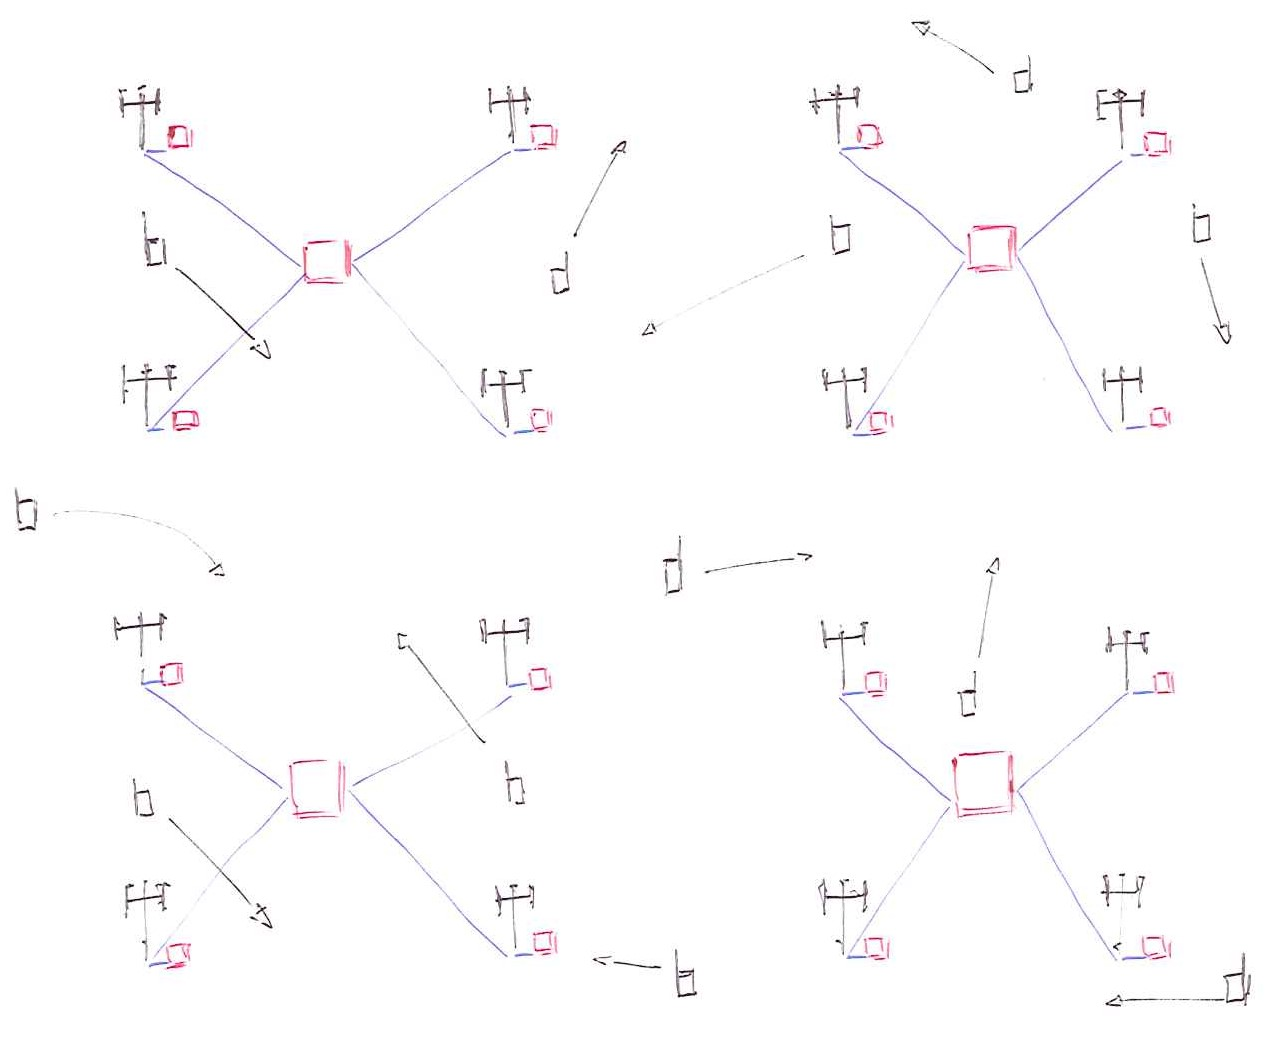
\includegraphics[width=\linewidth]{performance_delay.jpg} 
	\caption{Performance model}
	\label{fig:performance_model}
\end{figure}

As the the topology of the \xcloud and future mobile networks is yet to be determined, and due to the fact that we want to research the effects of mobility without a socio-economic model, the network 

%------------------------------------------------------------------

\section{Simulation model}

\subsection{Service}
Most mobile applications use HTTP as a means to communicate with remote services, often through a web interface \cite{maier2010first,falaki2010first}. We will model our service application to that of a stateless web service catering to the subscribers in the local network. The HTTP traffic model in \cite{reyes1999page} provides an open loop traffic model with a long tailed session size distribution, representative of the diversity of mobile the requests. 

Each session is separated in time with a poisson process of $\lambda_{ses}$. Each session produces $N_{req}$ requests, sampled from an inverse Gaussian distribution, where each request is separated in time by log-normal distributed delay $D_{req}$. See Figure \ref{fig:traffic_model}.

\begin{figure}[tb]
	\centering
	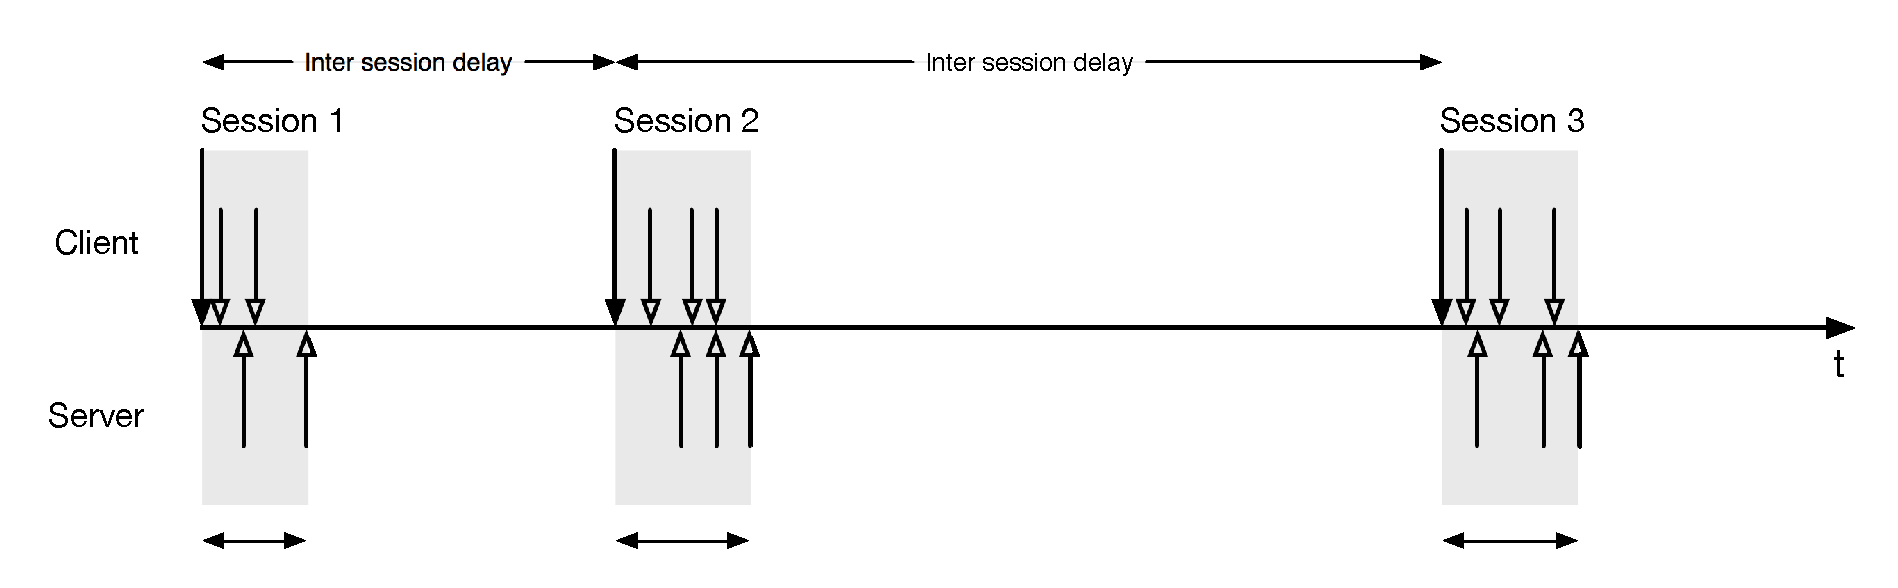
\includegraphics{fig_traffic_model.eps} 
	\caption{Traffic model fundamentals}
	\label{fig:traffic_model}
\end{figure}

Each service adheres to the same properties, and are only distinguished by the \ac{VM} in which they are running. Additionally, the properties of the service model are independent of \ac{MD} state and mobility mode.

% Even older ; reyes1999page
\subsection{Mobility}
The 2-dimensional, multi modal, mobility model \cite{bettstetter2001smooth} will provide the uniform mobile network with a relevant distribution of users.
\subsection{Mobile access network}
Forthcoming cell plannig practices will aim increase area energy efficieny by favouring smaller cells in urban areas \cite{shahab2013framework,5360741}. The model will therefor employ a small homogenous mobile network composed of $N_{rbs}$ radio base stations equidistantly distributed. The domain which the network serves is populated by a homogenous group \ues, with a uniform service subscription distribution. A \ue{} is handed over between base stations at the point where they cross the cell boundary distinguishing two independent radio base stations defined by the width of the rectangular cells $d_{rbs}$. The mobile access network model does take into account the physical layer, channel provisioning, and cell load balancing. Additionally, the radio access network functions as a mechanism to associate \ues{} with \dcs{}, propagation and system processing delays are thus not modelled.
\subsection{Core network}
The delay induced by the core network is modelled with a Weibull delay $T_{net}$ in multiples of the number of network nodes between the source and the destination, in accordance with \cite{papagiannaki2003measurement}. The distance between \rbss{} is equal to the cell dimension $d_{rbs}$. Associated \rbss{} are equidestant to their common \dc{}, and are for the sake of simplicity assumed to be separated by one router.
\subsection{\Dc}
\begin{figure}[tb]
	\centering
	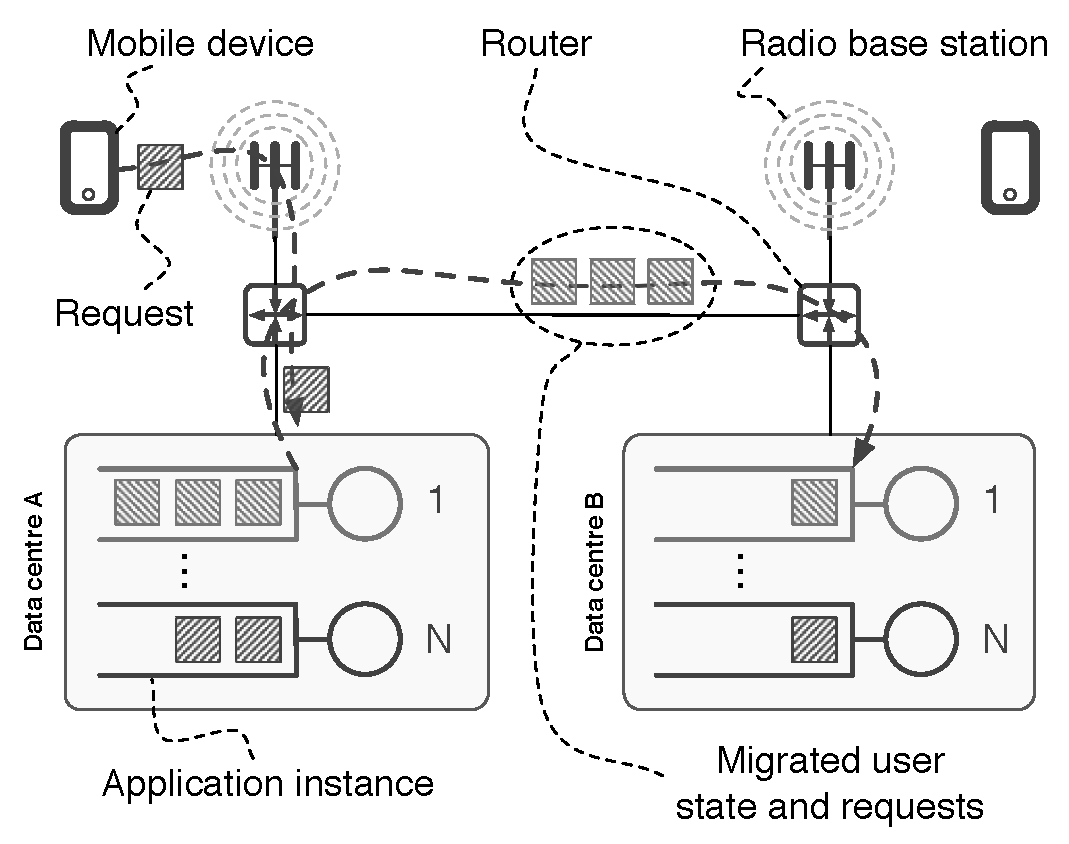
\includegraphics[width=\linewidth]{fig_dc_model.eps} 
	\caption{\Dc{} model}
	\label{fig:dc_model}
\end{figure}

As illustrated in Figure \ref{fig:dc_model}, a \dc{} is modelled as a series of parallel queues, one for each hosted VM.
%As illustrated in Figure \ref{fig:dc_model}, a \dc{} is modelled as a series of parallel queues, one for each allotted VM, and thus, service $N_{i,vm}$. 
%A dispatcher directs incoming requests to the corresponding VM based on which service $S_j$ it carries. 
%In normal operation, each request is served by its associated queue with a service time of $T_{i,vm}$, unique to the $i_{th}$ \dc{} and is proportional to the number of VMs $N_{i,vm}$ running concurrently in the \dc{} in excess of $N_{ser}$.
%When the queue in a VM or subset of VMs in a \dc{} $N_{i,sus vm} \subset N_{i,vm}$ are temprarily empty, the remaining VMs will be rewarded with a reduction in service time propotinal the number of suspended VMs $T_{sus} \propto N_{i,sus vm}$.

To simplify the model of a \dc{} we do not consider CPU, memory, storage and intra \dc{} network separately.
Instead, in this paper, we will use an abstraction of one dimensional computational resource.

\subsubsection{Hosting VMs in a \dc{}}
%Hosting VMs in a \dc{} can be modeled in two ways: with or without competition for computational resource.

%In the first approach, the resources of a \dc{} are aggregated in one pool that is continuously divisible.
%Each VM gets an equal part of available resources inversely proportional to the number of VMs hosted in the data center.
%The bigger is the number of VMs hosted in the \dc{}, the smaller amount of resources each of them gets.
%The pool of resources is divided evenly among all VMs.
%Hence, when the number of VMs hosted in the \dc{} increases, the amount of resources available for each VM shrinks.
%Consequently the service time of processing requests of each VM lengthens.

%In the second approach, the resources of a \dc{} are discrete and each computational unit is used exclusively by one VM.
%Therefore, there is no influence of one VM on another.
%To incorporate the fact that the amount of resources is finite we put a limit on the maximal number of VMs that can be hosted in one \dc{}.
%Furthermore, on each \dc each service is contained within one VM. 

Limitation of the number of hosted VM

Strong limit --- new VMs not accepted when the nominal capacity of DC is reached 

Flexible --- when the nominal capacity of DC is reached accepting new VMs causes increase of the service time

\begin{equation}
T_{serv} = \frac{max \lbrace nominal\_DC\_capacity, \#VMs \rbrace}{\#VMs} \cdot basic\_service\_time
\end{equation}

%\subsubsection{Overhead of VM start, stop, and migration}
%\subsubsection{Overhead of VM initialization and migration}
\subsubsection{VM initialization and termination}
%When a request from a previously unknown service $S_j$ is served to a \dc{}, a new VM will be started to host that service.
When a decision of deploying a new service in a \dc{} is taken, a new VM will be started there to host that service.
Due to the startup time, the newly admitted VM will not be able to start processing requests for a period of $T_{vm\_init}$. 
%Nevertheless, the base VM service time for the \dc{} $T_{i,vm}$, will be adjusted to the for the new VM count.
Nevertheless, the new VM will start using resources of the \dc{} from the time of admission.
Because of that, the service time, $T_{i,vm}$, for each of the VMs hosted in that \dc{} will be recalculated to reflect the temporary load scenario.
Similarly, after finishing serving the last request, the VM will still be using the resources of the \dc{} for time $T_{vm\_release}$.

\subsubsection{VM activation scheme}
Definitions: service, session, client subscribed to service 

%\begin{enumerate}
%	\item Private VM
\textbf{Private VM} --- IaaS like, a VM is exclusively used by one user for offloading computations from his \ue{}.
User provides the executable program that is loaded to an edge \dc{} from an \ue{} or a remote \dc{}.
		\begin{description}
			\item \textbf{per-session} --- a VM is initialized upon receiving the first request from a client and terminated just after finishing processing the last request of the session.
			\item \textbf{client-within-cell} --- a VM is initialized when a client that is subscribed to a service enters a cell and is kept alive as long as he stays within the cell. 
		\end{description}
			
%	\item Shared VM
\textbf{Shared VM} --- SaaS like, a VM hosts a service that can be concurrently accessed by many users.
		\begin{description}
			\item \textbf{any-client-running} --- a VM is initialized upon receiving the first request from a client and terminated when there are no more requests to serve (waiting queue is empty and all sessions are finished).
			\item \textbf{any-client-within-cell} --- a VM is initialized when the first client that is subscribed to a service enters a cell and is kept alive as long as any subscribed client stays within the cell. 
		\end{description}
%\end{enumerate}

\subsubsection{VM migration}
Migration has an influence on the service performance as well as on the resource availability on both source and destination \dc{}.
On the source side, apart from ordinary resource requirements due to serving requests, VM consumes resources for sending its image to the destination \dc{}.
In a case of postcopy live migration, VM at the source side still uses some resources even after the workload is redirected to the new location.
That is because the VM at the destination side pulls remaining memory pages from the source \dc{}.

%The overhead of VM migration can be modeled in different ways depending on the manner how \dc resources are represented.

To model the overhead of migration on the service performance additional delay in the response time should be introduced.
%Primarily, during the phase of transferring the image of VM, because of using a part of resources for I/O operations.
Primarily, for the time of transferring the image of VM, $T_{vm\_transfer}$, the time of serving a request should be lengthen by $D_{vm\_transfer}$, because of using a part of resources for I/O operations.
Moreover, during the time of switching the execution from the source to the destination, $T_{vm\_downtime}$, VM is not able to serve any requests.
%Additionally, in the case of the postcopy migration, delay occurs also for some time after redirecting the workload to the new \dc{}, due to the remote memory calls.
Additionally, in the case of the postcopy migration, delay  $D_{memory\_pull}$ occurs for some number, $N_{memory\_pull}$, of the first requests after redirecting the workload to the new \dc{}, due to the remote memory calls.

%That can be modeled by running two instances of VM during the time of migration, one per each DC.
When VMs compete for resources, running additional VM on the destination side introduces an overhead by increasing the response time of other collocated VMs.

%------------------------------------------------------------------

\section{Results}

%------------------------------------------------------------------

\subsection{Conslusions} 

%------------------------------------------------------------------

\section{Future research}

\begin{itemize}
\item \Dc{} provisioning and service/VM migration/placement schemes in the \xcloud{}.
\item Multi-tierd service placemet scehemes in the \xcloud{}.
\end{itemize}

%------------------------------------------------------------------

\bibliographystyle{plain}
\bibliography{references}

\end{document}